\documentclass[11pt]{article}
\usepackage{graphicx}
\usepackage{caption}
\usepackage{subcaption}
\usepackage[a4paper, portrait, margin=1in]{geometry}

\usepackage{mathtools}
\DeclarePairedDelimiter{\ceil}{\lceil}{\rceil}

\begin{document}

\title{Advanced Systems Lab (Fall'16) -- Second
Milestone}

\author{Name: \emph{Aleksander Matusiak}\\Legi number: \emph{16-931-925}}

\date{
\vspace{4cm}
\textbf{Grading} \\
\begin{tabular}{|c|c|}
\hline  \textbf{Section} & \textbf{Points} \\ 
\hline  1 &  \\ 
\hline  2 &  \\ 
\hline  3 &  \\ 
\hline \hline Total & \\
\hline 
\end{tabular} 
}

\maketitle

\newpage

\section*{Notes on writing the report \small{(remove this page for submission)}}

Before starting to work on this milestone please remember:
\begin{itemize}
\item The prerequisite to a successful completion to this milestone is to have a stable system and also the necessary logging functionalities in place. 
\item Depending on the workload and goal of the experiment, you might need to change the sampling rate from the default level. Make sure to indicate when doing so.
\item The choice of experiment length and repetitions is up to you to decide, please make sure that you do not include warm-up and cool-down phases in the measurements. There are many experiments to run in this milestone, try to make a tradeoff.  
\item We recommend that you have scripts in place to deploy and run experiments.
\item All experiments have to be executed on the Microsoft Azure cloud.
\item When plotting graphs include errors or measures of accuracy whenever possible. 
\item Keep the report compact and concise! The total length should not exceed 20 pages. Log listings are not counted in this length, but all text, figures and tables are. If you have many logs, compress them by experiment and reference the archive instead of the independent files.
\end{itemize}

In this milestone we expect to see the different experiments you ran to exercise the system, and with each experiment we expect a clear description of the system configuration used, the hypothesis on behavior and the explanation of the behavior observed (in terms of the different design decisions taken beforehand) -- \emph{missing either of these for an experiment might make you lose all points for that given experiment!} 

Keep in mind that for a good explanation of the results of an experiment you might have to use one or more methods of data analysis presented in the lecture and in the book. You might have to combine measurements taken in the middleware with the ones at the clients to be able to provide a full picture.

Please feel free to structure the three sections of this report as it makes most sense for your experiments and explanations, but please respect the goal of each section. Also, similarly to the first milestone, include tables and descriptions about your experimental setup before each set of experiments.


\pagebreak

\section{Maximum Throughput}
\label{sec:max-throughput}

%Find the highest throughput of your system for 5 servers with no replication and a read-only workload configuration. What is the minimum number of threads and clients (rounded to multiple of 10) that together achieve this throughput? Explain why the system reaches its maximum throughput at these points and show how the performance changes around these configurations. Provide a detailed breakdown of the time spent in the middleware for each operation type.

\subsection{Hyphotesis}

The throughput, as we increase the number of clients, should be increasing, at least to the point where my middleware encounters problem. However, as we could already see on the plot for baseline experiment in the milestone 1, the mean response time shall increase almost in a linear way. This means that the maximal effective throughput will be probably achieved for not that big number of clients - for higher number of clients throughput will probably still increase slightly, but the response time would increase much faster.

The throughput, as we increase the number of threads in the thread pool, should also be increasing. However, creating more threads is associated with more overhead from operating system and might not improve the throughput as much as we would expect. 

I predict that the bottleneck for the middleware would be the receiving of incoming client requests and putting them into an appropriate queue, since it is performed by only one thread, while every other operation can be executed by multiple threads in parallel. This means that at some points increasing the number of threads in the thread pool would not affect the throughput significantly - it will be limited by the bottleneck, which isn't affected by the increase of threads.
%TODO 

\subsection{General experimental setup}
Using memaslap in the read-only configuration means that before actual statistics are being displayed there is a phase where each memaslap clients sends only set requests in order to fill up the server with some keys, which it can later query. This face was initially taking a very longs time due to the default window size. Therefore, for all the experiments in this task I have decreased the window size for each memaslap client to 1k, which made initial phase with only set requests much shorter (lasting less than one minute). However, different servers still could finish initial phase much before others. Therefore, to be sure that during actual measurement all memaslap servers are sending only get requests, I have conducted the experiments for 5 minutes and for calculating statistics I have used only the third minute. This means 2 minutes for warm up phase and 2 minutes for cool down phase, which includes waiting with measurements for other servers to stop sending set requests. I have collected statistics every second. This means that for each configuration I have collected 60 numbers, from which I could calculate average, standard deviation and, when applicable, percentiles. Due to the limit of money I was able to use for this milestone (my subscription was renewed on 1st November), I couldn't afford repetition of the experiment. Even though I was left with some funds near the end of the milestone, conducting repetition experiments not immediately after the original one, would not give any positive contribution for my experiments, since the results would differ significantly due to uncertainty of the Azure cloud. However, I strongly believe that collecting 60 values for each configuration, as described above, provides statistical significance for my experiments.   

To avoid memcached misses I have increased the memory of each memcached server to 256 MB.

In order to enable distinction between between set and get requests in the middleware logs, I have added writing the type of request for every log entry. What is more, with higher number of clients, my middleware was sometimes not forwarding received requests and responses correctly. This was due to not checking for emptiness of the buffer after sending the first part of the message - sending should be continued till the buffer is empty. This bug was fixed in the source code and corrected code was used for running the experiments for this milestone. 

\subsection{Overall experiment}
This experiment was conducted using the following provided scheme:
\medskip

\small{
\smallskip
\begin{tabular}{|c|c|}
\hline Number of servers & 5 \\ 
\hline Number of client machines & 5 \\ 
\hline Virtual clients / machine & 20 - 100 \\ 
\hline Step for virtual clients / machine & 10 \\ 
\hline Threads in the thread pool & 10 - 60 \\
\hline Step for threads in the thread pool & 10 \\
\hline Workload & Key 16B, Value 128B, Writes 0\% \\
\hline Middleware & No replication \\ 
\hline Runtime x repetitions & 5 min x 1 \\ 
\hline Warm-up phase & 2 min \\
\hline Cool-down phase & 2 min \\

\hline Log files & overall1, overall2, overall3, overall4, overall5, overall \\
\hline 
\end{tabular} }
\medskip


\begin{figure}
\centering
\begin{subfigure}{.5\textwidth}
	\centering
	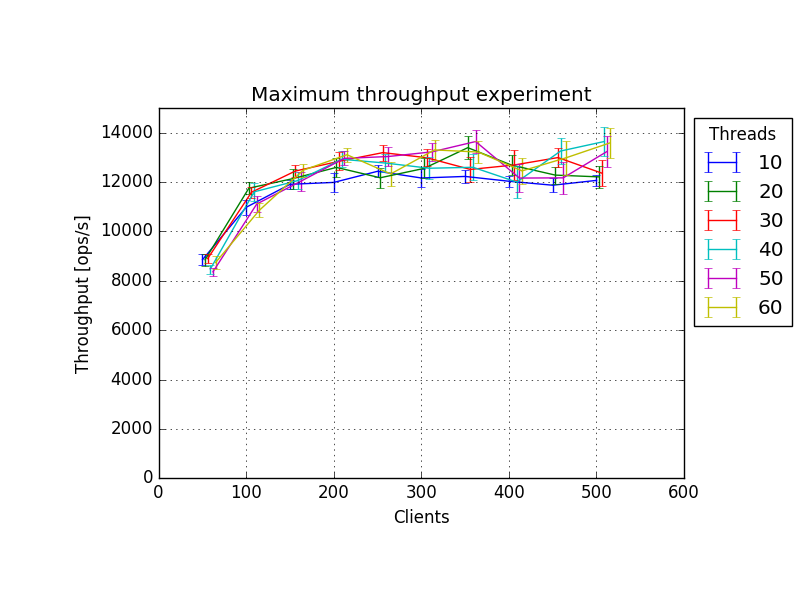
\includegraphics[width=\linewidth]{plots/max_throughput_all_overall}
	\caption{Throughput}
\end{subfigure}%
\begin{subfigure}{.5\textwidth}
	\centering
	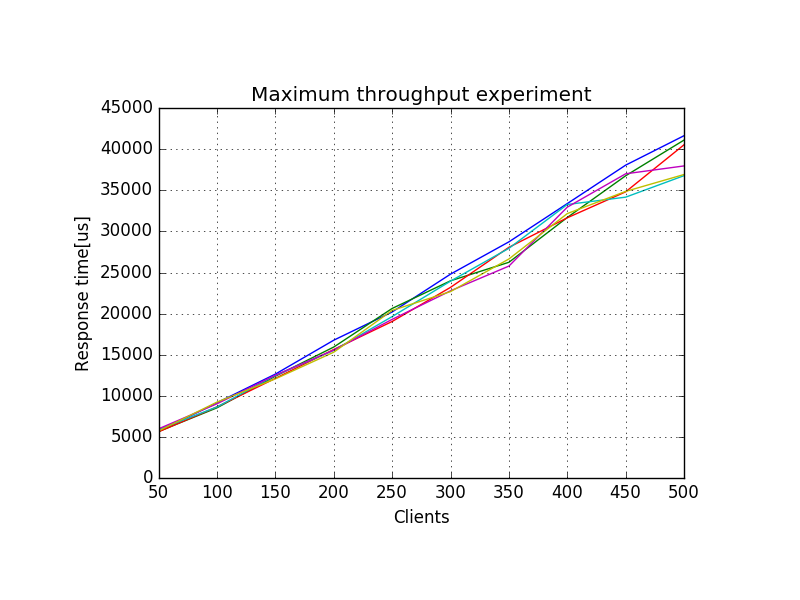
\includegraphics[width=\linewidth]{plots/max_throughput-response_time_all_overall}
	\caption{Response time}
\end{subfigure}
\caption{Plots for various number of threads in the overall experiment}
\label{fig:max-throughput-overall}
\end{figure}

Results of this experiments are visible in the figure \ref{fig:max-throughput-overall}.

As we can see from the plots, the throughput up to 500 clients is slightly growing. However, the response time is also growing in almost linear manner. This means that the maximal effective throughput should be achieved by clients in range around 150 - 250 clients. More precisely, the highest throughput for my experiment was achieved using 500 clients and 40 threads in the thread pool - it was equal to 13648 ops/s and it was corresponding to mean response time equals to around 36790 us. If we look at the range 150-250 clients, the highest throughput was achieved for 250 clients and 30 threads - it was equal to 13196 ops/s and it was corresponding to mean response time equals to around 19057 us. This means that by limiting our analysis to range till 250 clients, we get highest throughout worse by around 3,3\%, but the response time is around 48,2\% lower (better). This means that we can indeed concentrate on the number of clients till 250, since the increase of the number of clients above it will maybe slightly increase throughput, but the response time will grow significantly.

% TODO: interactive law

It must also be pointed out here that number of threads does not make such a big difference as one could expect. We can clearly see in the plot that the middleware having 10 threads in each of the thread pool is performing noticeably worse then the middleware having more threads. We can still see that below 300 clients the middleware with the thread pool of size 20 is performing less effective than with other configurations. However, for bigger number of clients and size of the thread pool, difference in performance is not really significant. Therefore, as the optimal number of threads I have chosen 30 threads, since lower number of threads results in noticeably lower performance and higher number of threads does not make a significant difference. The reason why this is the case is probably the bottleneck for the middleware is receiving incoming requests from the clients, not forwarding them to servers. This will be thoroughly analyzed in the subsection \ref{sec:time-breakdown}. What is more, the reason for not big effect of the number of threads might be the overhead from operating systems. Having more threads costs some system resources and since the virtual machine has only 8 cores, the threads might not be in reality performing task in parallel, but rather one after another.

\subsection{Detailed experiment}

This experiment was conducted using the following provided scheme:
\medskip

\small{
\smallskip
\begin{tabular}{|c|c|}
\hline Number of servers & 5 \\ 
\hline Number of client machines & 5 \\ 
\hline Virtual clients / machine &  20 - 60 \\ 
\hline Step for virtual clients / machine & 2 \\
\hline Workload & Key 16B, Value 128B, Writes 0\% \\
\hline Middleware & No replication \\ 
\hline Runtime x repetitions & 5 min x 1 \\ 
\hline Warm-up phase & 2 min \\
\hline Cool-down phase & 2 min \\
\hline Log files & TODO \\
\hline 
\end{tabular} }
\medskip

\begin{figure}
\centering
\begin{subfigure}{.5\textwidth}
	\centering
	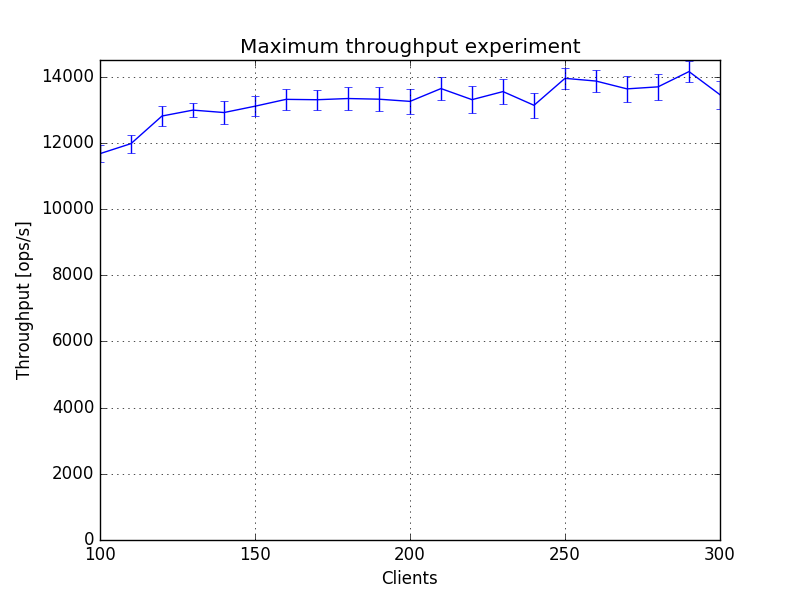
\includegraphics[width=\linewidth]{plots/max_throughput_all_detailed}
	\caption{Throughput}
\end{subfigure}%
\begin{subfigure}{.5\textwidth}
	\centering
	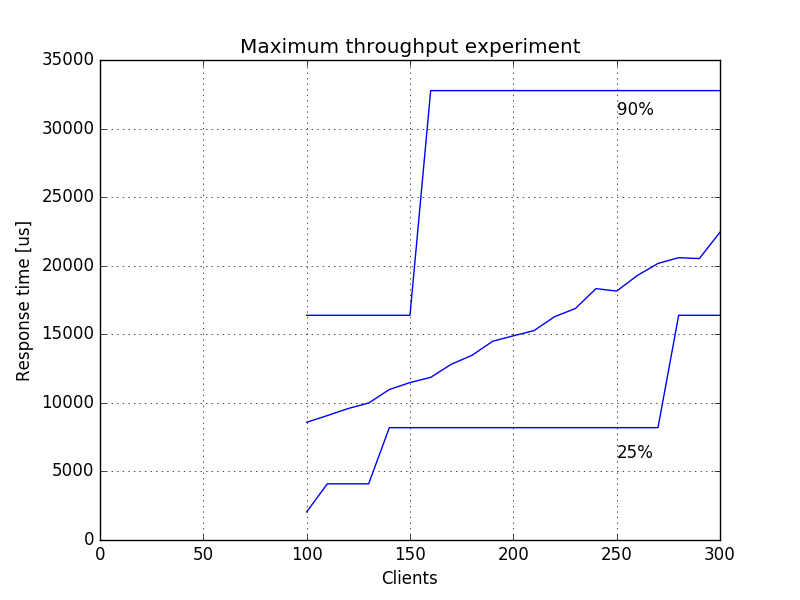
\includegraphics[width=\linewidth]{plots/max_throughput-response_time_all_detailed}
	\caption{Response time}
\end{subfigure}
\caption{Plots for various number of threads in the detailed experiment}
\label{fig:max-throughput-detailed}
\end{figure}

Results of this experiments are visible in the figure \ref{fig:max-throughput-detailed}.


To sum up, the maximal effective throughput is achieved for 210 clients and size of thread pool equals 30. Therefore, I will use this parameters in later experiments.  

\subsection{Verification of the hyphotesis}

As I have suspected, the number of clients for the maximal effective throughput was not that big and increasing number of clients further would only cause a slight increase in the throughput and a more significant increase in the mean response time. Further increasing of threads above 30 threads, as predicted, does not contribute to the higher throughput.

\subsection{Breakdown of the time spent in the middleware}
\label{sec:time-breakdown}

Since the purpose of this experiment was to analyze middleware under read-only workload, in this section I will provide breakdown of the time spent in the middleware for get operations.
\medskip

\begin{tabular}{|c|c|c|c|}
\hline \bf{Time spent ...} & \bf{Average (us)} & \bf{Standard deviation (us)} & \bf{Coefficient of variation} \\ 
\hline in the middleware & 6931 & 12213 & 1.76 \\
\hline in the queue & 2678 & 7192 & 2.69\\
\hline in the server & 4203 & 9329 & 2.22\\
\hline in the queue and the server & 6881 & - & -\\
\hline being actively processed & 50 & - & -\\
\hline
\end{tabular}
\medskip

As we can see from the above table, most of the time (almost 61\%) is spent by the requests in servers (which means - being transferred via network to and from server and being processed by the server). Time spent in the queue is less significant (around 39\%). This is because we have chosen optimal number of threads to achieve the best performance. With 30 threads in the single thread pool (for each server), so in total with 150 threads processing get requests, we can process requests from 210 clients effectively. However, we must remember that the processor on the virtual machine on which the middleware server was running, has only 8 cores. Therefore, time waiting in the queue is not negligible and influences the total time spent in the middleware.

It must be pointed out that the coefficient of variation for time spent in the queue is high, also comparing to time spent in the servers and total time in the middleware. This is because time spent in the queue depends also on other factors. If we have some disturbance in the network, threads processing get requests will have to wait longer for response from the server and therefore will not be able to take next requests of out the queue. What is more, if there is disturbance in the network from client to the middleware server, workers might be idle, whereas when later huge number of requests come, they will not be able to process the effectively. This means that time spent in the queue depends significantly on other factors, which explains why it can vary noticeably.  

\pagebreak

%-----------------------------------------------------------

\section{Effect of Replication}

\iffalse
Explore how the behavior of your system changes for a 5\%-write workload with S=3,5 and 7 server backends and the following three replication factors:
\begin{itemize} 
\item Write to $1$ (no replication) 
\item Write to $\ceil{\frac{S}{2}}$ (half) 
\item Write to all 
\end{itemize}

Answer at least the following questions: Are \texttt{get} and \texttt{set} requests impacted the same way by different setups? If yes/no, why? Which operations become more expensive inside the middleware as the configuration changes? How does the scalability of your system compare to that of an ideal implementation? Provide the graphs and tables necessary to support your claims.
\fi

\subsection{Hyphotesis}
\label{sec:replication-hyphotesis}

As we increase the replication factor (number of servers to which we send each set request), the performance of the middleware should decrease. This is quite obvious - we have to send more set requests to servers and then receive and process all the replies. What is more, server will become more overloaded, which might also lower the performance of the system. With higher replication factor we should also have higher variation of the data, since we will be more prone to network latencies. Behavior described in this paragraph should be mostly visible for set requests, but since they consist of 5\% of the requests, it shall also affect overall performance. I predict that the replication should not influence significantly the time spent in the middleware for get requests since replication configuration changes change only how set workers perform their tasks. However, the middleware will have to perform more actions, which might slightly affect response time also for get requests. 
% TODO is this true?

% TODO: hyphothesis about increase of servers

\subsection{Experimental setup}

\small{
\smallskip
\begin{tabular}{|c|c|}
\hline Number of servers & 3 - 7 \\ 
\hline Step for number of servers & 2 \\
\hline Number of client machines & 3 \\ 
\hline Virtual clients / machine &  70 \\ 
\hline Workload & Key 16B, Value 128B, Writes 5\% \\
\hline Middleware & Replication: none, half, all \\ 
\hline Runtime x repetitions & 3 min x 3 \\
\hline Warm-up phase & 1 min \\
\hline Cool-down phase & 1 min \\
\hline Log files & TODO \\
\hline 
\end{tabular} }
\medskip

\subsection{Overall performance}
\label{sec:replication-overall}

\begin{figure}
\centering
	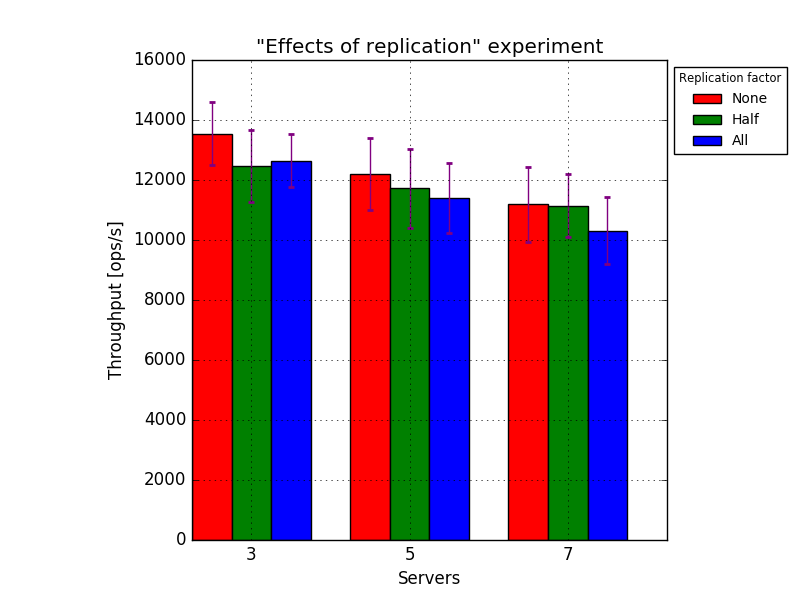
\includegraphics[width=0.7\linewidth]{plots/replication}

\caption{Aggregated throughput for the replication experiment}
\label{fig:replication-overall}
\end{figure}

% TODO what does performance mean - throughput / time spent, interactive law

As we can see from figure \ref{fig:replication-overall}, performance of the system (measured as the throughput) for 5 and 7 servers is decreasing as we increase the replication factor. For 3 servers we can also notice that as we increase replication factor from none to half, the performance decreases, but when we increase the replication factor from half to all we can notice a slight increase of the performance. However, the difference between these values is within statistical error.
% TODO can I do that?

The performance of the middleware as we increase the replication factor was predicted properly in the section \ref{sec:replication-hyphotesis}. However, we can't notice the change in standard deviation of the throughput as we increase replication factor. This might be because we measure throughput every second, so although we can get differences in performance within one second, they are smoothen out when we take the measurement from the whole second. The variation of data will be further analyzed in section \ref{sec:replication-set}, where we can get more accurate data as far as distribution of data is concerned.

From the plot we can also see that the performance decreases as we increase the number of servers (for every replication factor). As we go from 3 to 7 servers we notice decrease in the performance (throughput) of 17\%, 11\% and 18\% for replication factor: none, half and all respectively. With more servers we create more threads, which causes more overhead to our middleware. With only 8 cores available on the virtual machines, higher number of threads might cause threads fighting over processor resources, which leads to reduce performance. Although load for each server is lower with higher number of servers, the bottleneck of the whole system is middleware and overhead on the middleware causes lower performance.

\subsection{Scalability of the system}
% TODO: what does ideal scalability mean?
Following the analysis presented in the section \ref{sec:replication-overall}, we can conclude that our system does not provide good scalability. As we increase number of servers in the ideal system, the performance of the system should increase, since there would be less load on each server. However, the experimental result show completely opposite behavior - as we increase the number of servers, performance lowers. This enables us to conclude that memcached servers are not saturated and it is our middleware that is the bottleneck of the system. With more overhead on the middleware connected with more servers, we get noticeable worse performance.  


\subsection{Get requests}
\begin{figure}
\centering
	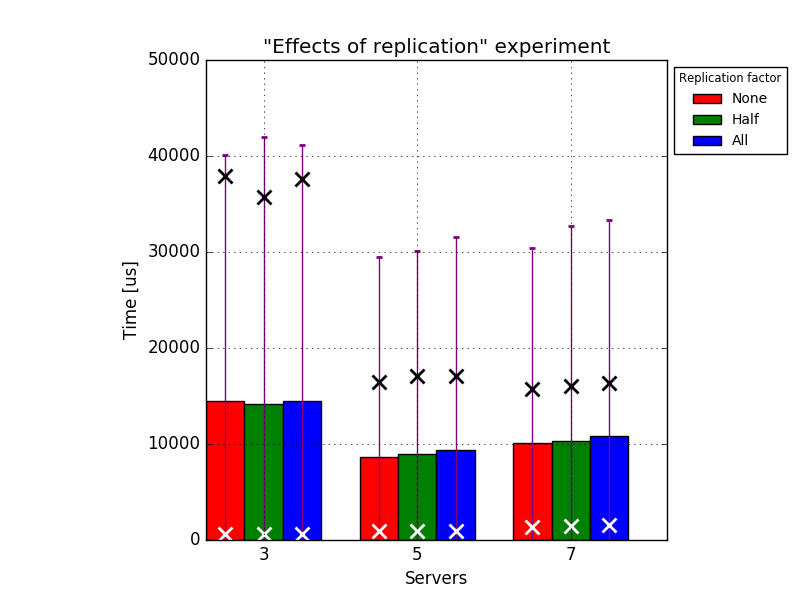
\includegraphics[width=0.7\linewidth]{plots/replication-get}

\caption{Total time spent in the middleware for get requests}
\label{fig:replication-get}
\end{figure}

We can see from the figure \ref{fig:replication-get} that get requests are not much affected by changing the replication factor. Differences between different replication factors are negligible, taking into the account how big is the standard deviation. This is because changing replication factor does not change the work that get workers have to do. There might be some additional load on the middleware connected with increased replication factor and also probably higher network traffic (more set requests), but as the plot shows, it does not matter that much for get requests. From figures \ref{fig:replication-get-queue} and \ref{fig:replication-get-servers} we also cannot see any significant difference in the time spent by the request for different replication factors.
%TODO overall time for different servers

% TODO: standard deviation discussion

% TODO: change y-axis labels
\begin{figure}
\centering
\begin{subfigure}{.5\textwidth}
	\centering
	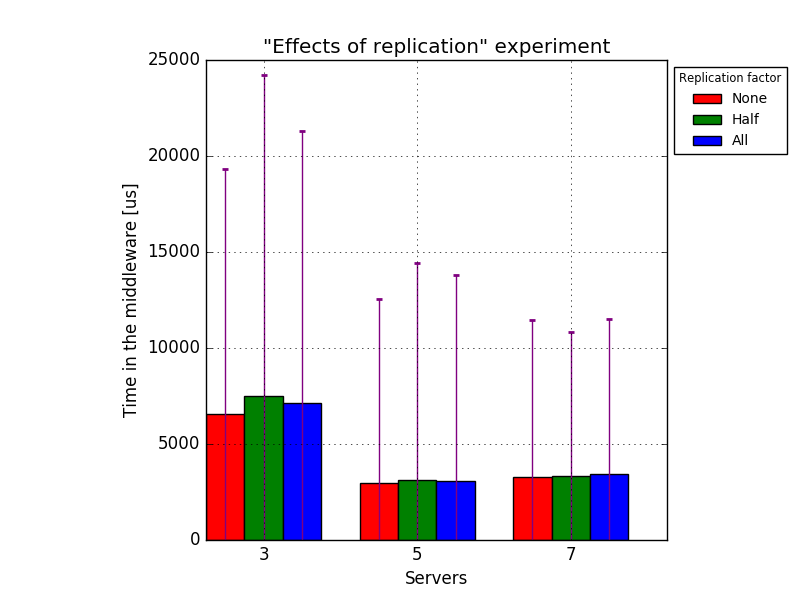
\includegraphics[width=\linewidth]{plots/replication-get-queue}
	\caption{Time in the queue}
	\label{fig:replication-get-queue}
\end{subfigure}%
\begin{subfigure}{.5\textwidth}
	\centering
	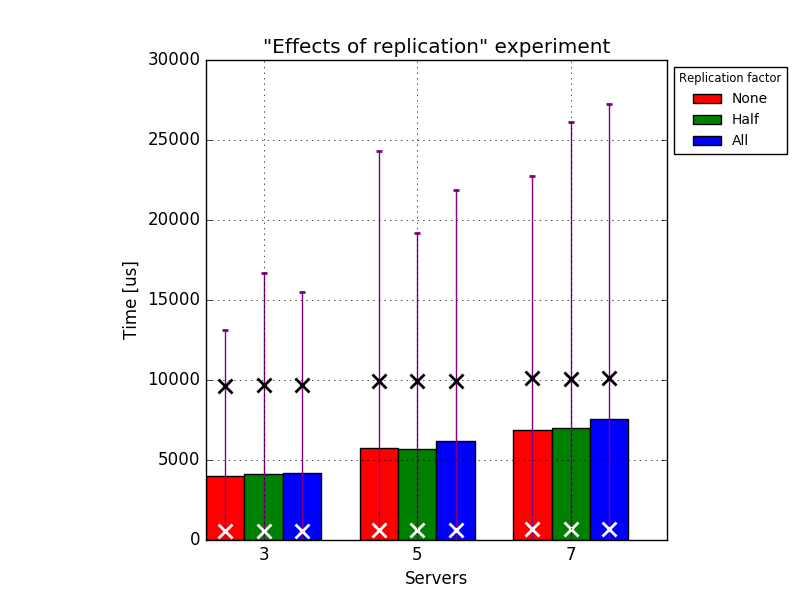
\includegraphics[width=\linewidth]{plots/replication-get-servers}
	\caption{Time in the servers}
	\label{fig:replication-get-servers}
\end{subfigure}
\caption{Breakdown of time spent in the middleware for get requests}
\label{fig:replication-get-breakdown}
\end{figure}


Looking at the figure \ref{fig:replication-get-queue} we can, however, see a significant difference in the time spent in the queue as we increase number of servers from 3 to 5. As we increase the number of servers from 3 to 5 we can see a decrease in time spent in the queue by around 57\%. This is because for 3 threads we do not have enough threads per request in the queue to allow to process threads from the queue efficiently. For 3 servers we have 70 requests and 30 threads per queue, we have $2\frac{1}{3}$ requests per thread. For 5 servers: 45 requests and 30 threads, which corresponds to $1\frac{1}{2}$ requests per thread. This means that elements can be taken out of the quickly for 5 servers, because each server has lower number of requests it has to process. However, when we increase number of servers from 5 to 7 we do not see a significant difference in this value. This means that decreasing number of requests per one queue would not further affect the time spent in the queue. This might be because starting from 1.5 requests per thread ratio the bottleneck of the system shifts to some other component, most probably to the thread accepting incoming requests.

It is worth noticing here that his result is consistent with my results of experiments described in the section \ref{sec:max-throughput}. Increasing number of servers here decreases the ratio of requests per thread (for a given queue), while increasing number of threads (with constant number of requests) also decreased this ratio. In the section \ref{sec:max-throughput} we have concluded that number of threads in the thread pool equal to 30 is optimal. We used the same number of threads in this experiment. Therefore, increasing number of servers from 3 to 5 should correspond to increasing number of threads to 30 in the maximal throughput experiment, while increasing number of servers from 5 to 7 corresponds to increasing number of threads from 30 upward, which did not yield a noticeable difference.

When we look at the figure \ref{fig:replication-get-servers} we can see that increasing number of servers increases the time spent in the servers. This is because of more overhead from the side of the middleware - it takes longer to send and receive the message, as well as higher network traffic.
% TODO: really? do I measure time correctly?

\subsection{Set requests}
\label{sec:replication-set}
\begin{figure}
\centering
	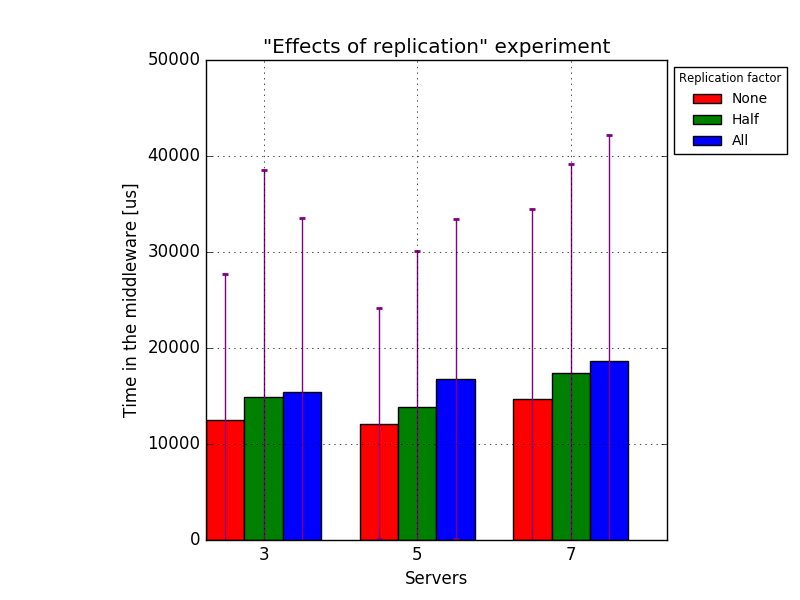
\includegraphics[width=0.7\linewidth]{plots/replication-set}

\caption{Total time spent in the middleware for set requests}
\label{fig:replication-set}
\end{figure}

%TODO overall time for different servers
%TODO: change elsewhere - must do more work
As we can see from the figure \ref{fig:replication-set}, increasing the replication factor increases noticeably the time spend by the set requests in the middleware. Setter worker with more servers to replicate to must collect responses from more servers and therefore is more prone to network latencies. More connections are established and if the one response takes longer than usual, it prolongs the total time of the request spent in the middleware. 

From the figure \ref{fig:replication-set-servers} we see that it is indeed time spend in the servers that influences the response time significantly. Changing of time in the queue is not relevant here (see figure \ref{fig:replication-set-queue}) - it is similar as we differ the replication factor. This can be explained in a following way: although we have only one setter thread, it takes the set request out of the queue quickly, because sending operation is asynchronous. This means, that sending operation itself, as well as collecting responses (using queue-like data structure used in my system and described in the report for milestone 1) is not really time-consuming. With more requests to send we do not notice worse performance of setter worker, since time spent in the queue does not differ significantly as we change the replication factor. We can therefore say that with higher replication factor setter worker itself performs similarly, but since we have more network requests to send and responses to receive we get worse performance, since we must wait for {\bf all} the responses and therefore we are more prone to network latencies.

% TODO: standard deviation discussion

\begin{figure}
\centering
\begin{subfigure}{.5\textwidth}
	\centering
	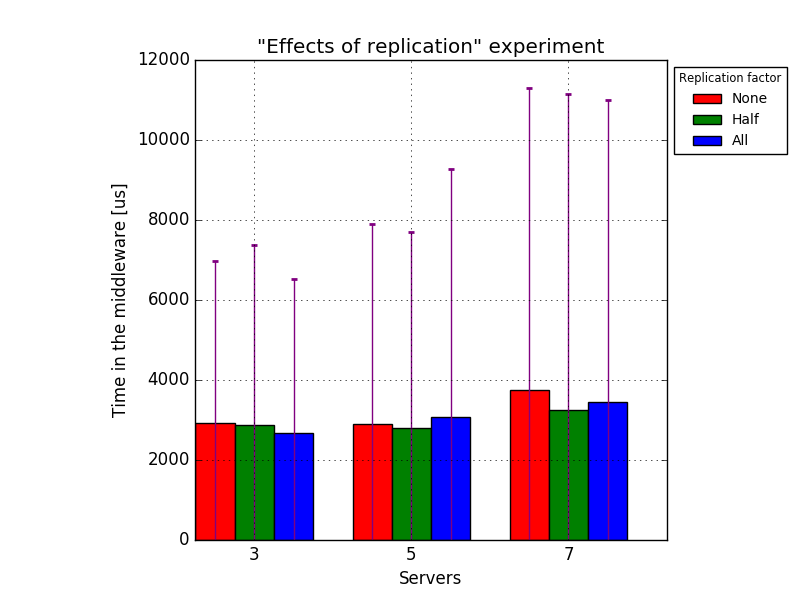
\includegraphics[width=\linewidth]{plots/replication-set-queue}
	\caption{Time in the queue}
	\label{fig:replication-set-queue}
\end{subfigure}%
\begin{subfigure}{.5\textwidth}
	\centering
	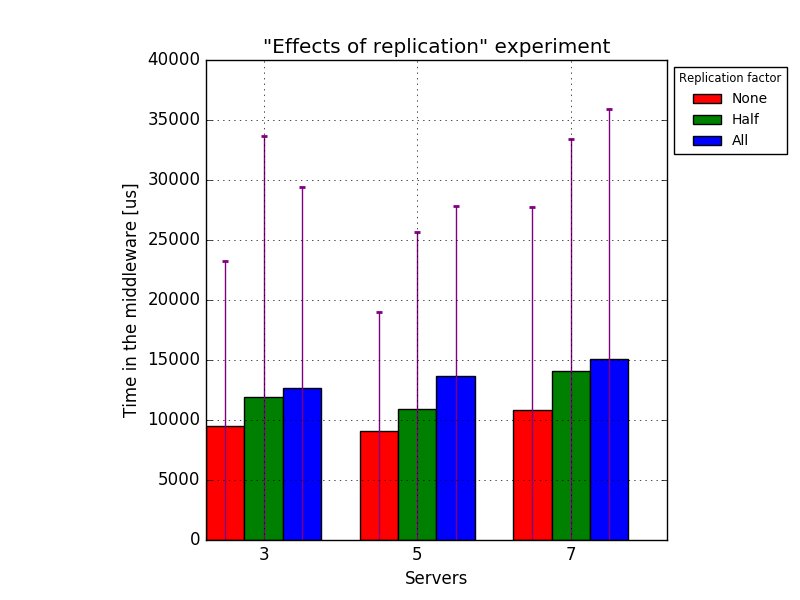
\includegraphics[width=\linewidth]{plots/replication-set-servers}
	\caption{Time in the servers}
	\label{fig:replication-set-servers}
\end{subfigure}
\caption{Breakdown of time spent in the middleware for set requests}
\label{fig:replication-set-breakdown}
\end{figure}

\subsection{Get vs set requests}

%TODO add appropriate plot/table?
Looking at the figures from previous section we can say that set requests spend more time in the middleware, especially when we increase the replication factor. Changing of the replication factor seems not to have a significant influence on times connected with get requests (overall time in the middleware, as well as in queue and in servers time). For set requests, however, more time is spent in the servers as we increase the replication factor, which results to higher overall time in the middleware (while time spent in the queue does not change significantly).

The impact of the amount of set requests will be analyzed thoroughly in the section \ref{sec:writes}

\subsection{Verification of the hypothesis}
My hypothesis was in a large part confirmed by the experimental results. Indeed increasing replication factor influences mostly set requests causing that they stay longer in the middleware. This also affects overall performance and average response time. However, performing more actions by the middleware did not affect the performance (as time spent in the queue for set requests does not change significantly).


\pagebreak

%-----------------------------------------------------------

\section{Effect of Writes}
\label{sec:writes}

In this section, you should study the changes in throughput and response time of your system as the percentage of write operations increases. Use a combination of 3 to 7 servers and vary the number of writes between 1\% and 10\% (e.g. 1\%, 5\% and 10\%). The experiments need to be carried out for the replication factors R=1 and R=all.  

For what number of servers do you see the biggest impact (relative to base case) on performance? Investigate the main reason for the reduced performance and provide a detailed explanation of the behavior of the system. Provide the graphs and tables necessary to support your claims.


\subsection{Experimental setup}

\small{
\smallskip
\begin{tabular}{|c|c|}
\hline Number of servers & 3 - 7 \\ 
\hline Step for number of servers & 2 \\
\hline Number of client machines & 3 \\ 
\hline Virtual clients / machine &  70 \\ 
\hline Workload & Key 16B, Value 128B, Writes: 1, 5 or 10\% \\
\hline Middleware & Replication: none, all \\ 
\hline Runtime x repetitions & 3 min x 3 \\
\hline Warm-up phase & 1 min \\
\hline Cool-down phase & 1 min \\
\hline Log files & TODO \\
\hline 
\end{tabular} }
\medskip



\begin{figure}
\centering
\begin{subfigure}{.5\textwidth}
	\centering
	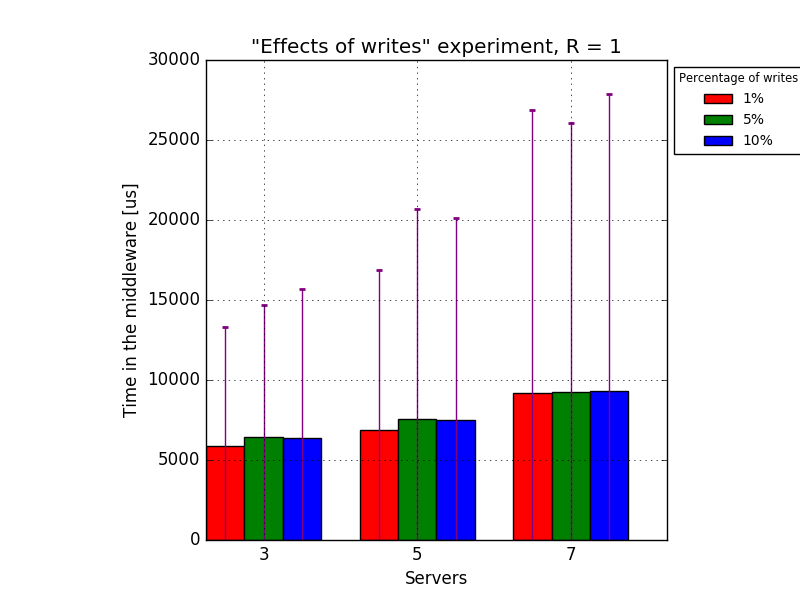
\includegraphics[width=\linewidth]{plots/writes-all-1-replication}
	\caption{Time in the queue}
	\label{fig:writes-all-1-replication}
\end{subfigure}%
\begin{subfigure}{.5\textwidth}
	\centering
	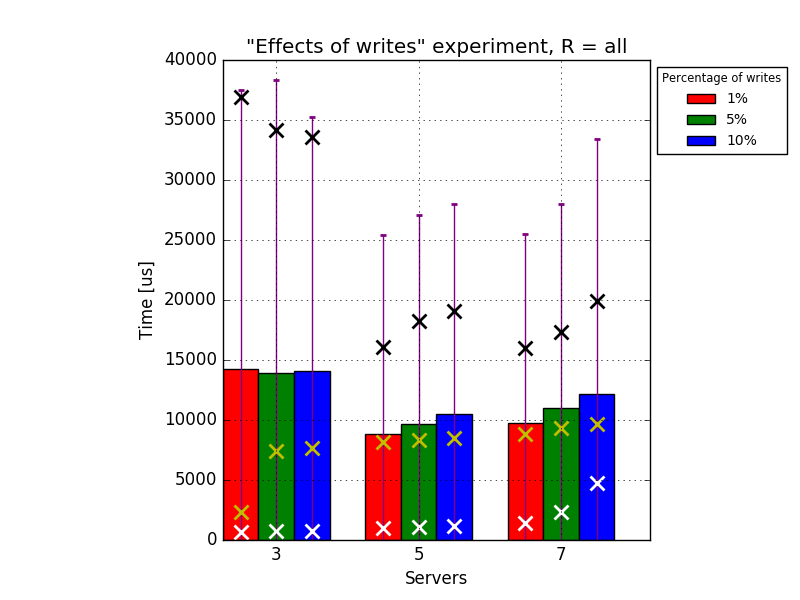
\includegraphics[width=\linewidth]{plots/writes-all-2-replication}
	\caption{Time in the servers}
	\label{fig:writes-all-2-replication}
\end{subfigure}
\caption{Breakdown of time spent in the middleware for set requests}
\end{figure}

 
\end{document}